% Provenance (never printed): old terminale S material on the early Earth (the
% primitive atmosphere and its outgassing, the first traces of life, the rise of
% oxygen read in the rocks: banded iron formations, red beds) and the faint young
% Sun. Owner (Sync 0/1): outgassing and primitive atmosphere, faint young Sun
% problem, stromatolite, Great Oxidation Event, banded iron formation, red beds.
% Recalled: age of the Earth (g12.07), zircons (g12.01), equilibrium temperature
% (g10.02), photosynthesis and cyanobacteria (biology), air composition, greenhouse
% gases as molecules and redox (chemistry). Figures: figdata/grade-12/early_earth.py.
\chapter{A Terra primitiva e a sua atmosfera}\label{ch:g12:early-earth}

Nas Hamersley Ranges, no noroeste da Austrália, as paredes do desfiladeiro
de Dales Gorge são listradas como um bolo em camadas: faixas finas de rocha
vermelha, cinza e preta. Elas são uma \omterm{def:g12:early-earth:bif}{formação ferrífera bandada}, depositada
num fundo marinho há mais de 2.5 bilhões de anos.
O ferro que elas contêm enferrujou nesse mar, e, para enferrujar, ele
precisou de oxigênio. Este capítulo pergunta como eram a Terra jovem e o seu
ar, e como as rochas registram o momento em que o oxigênio apareceu.
% ledger: dbca:karijini, earle:bif, photo:g12-dales-gorge

\begin{omfigure}
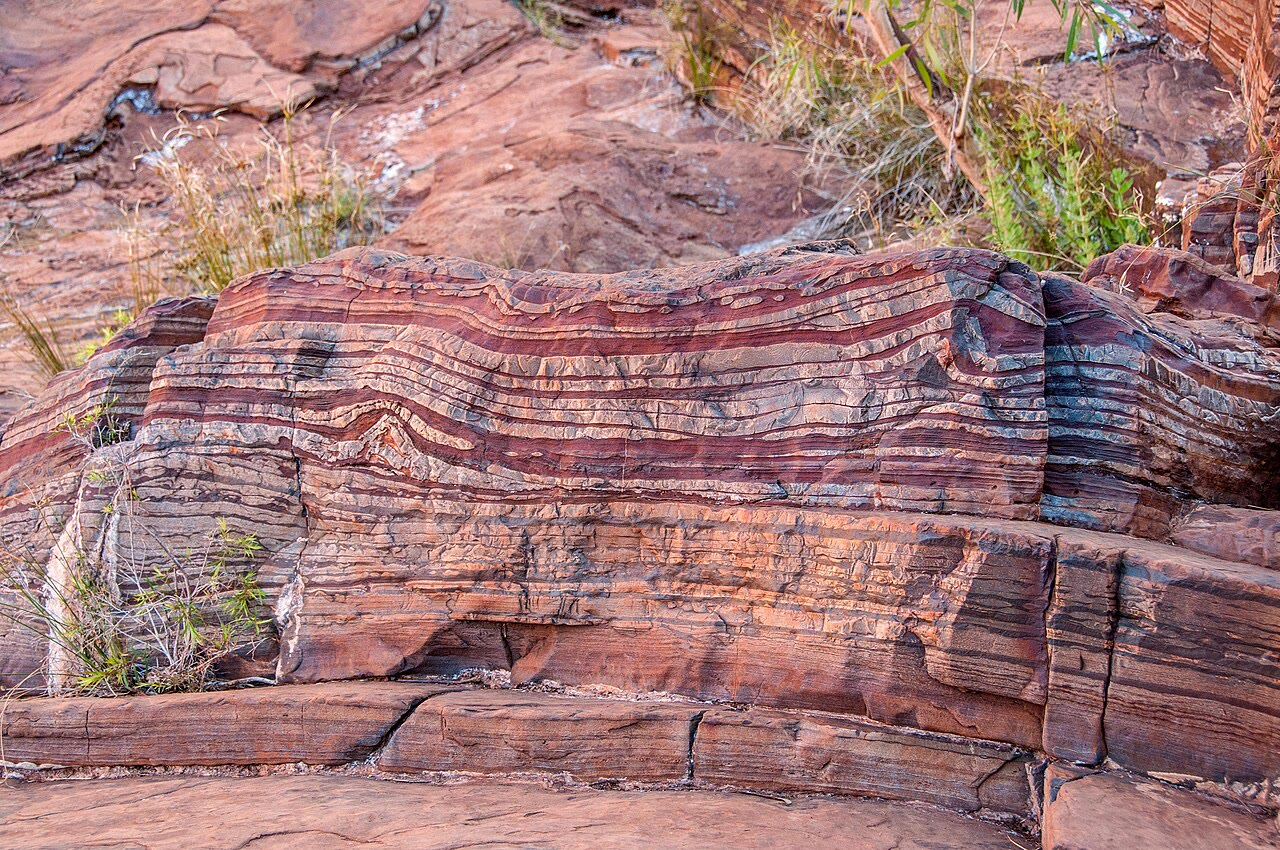
\includegraphics[width=0.72\linewidth]{images/book2/g12-dales-gorge-bif.jpg}

{\small \omterm{def:g12:early-earth:bif}{Formação ferrífera bandada} nas cachoeiras de Fortescue Falls, Dales
Gorge, Parque Nacional de Karijini, Austrália Ocidental. Fotografia Graeme
Churchard, CC~BY~2.0 (Wikimedia Commons).}
\end{omfigure}

\begin{recall}
A Terra tem 4.54 bilhões de anos (\cref{ch:g12:age-of-the-earth}), e os
zircões mostram que uma crosta existia há 4.4 bilhões de anos
(\cref{ch:g12:continental-crust}). A \omterm{def:g10:habitable-planet:equilibrium-temperature}{temperatura de equilíbrio} de um planeta,
$T_{\mathrm{eq}} = \left(S(1-A)/(4\sigma)\right)^{1/4}$, é de cerca de \qty{255}{K}
para a Terra de hoje (\cref{ch:g10:habitable-planet}). O ar seco de hoje tem
\qty{78}{\percent} de nitrogênio e \qty{21}{\percent} de oxigênio, e o gás
carbônico e o metano são gases de efeito estufa; um elemento que capta
oxigênio é oxidado (os livros de química). As plantas, as algas e as
cianobactérias fabricam o seu alimento pela fotossíntese, que libera
oxigênio (os livros de biologia).
\end{recall}
% ledger: usgs:age-earth (Book 1 row), wilde01:zircon, earth:TSI, earth:albedo, air:N2, air:O2

\section{A Terra jovem}

A Terra cresceu pela acreção de corpos menores. Cerca de 60 milhões de anos
depois que o Sistema Solar começou a se formar, um corpo talvez do tamanho
de Marte a atingiu, e o material lançado no espaço formou a Lua. A Terra
jovem era quente e ainda em parte fundida. Ela esfriou, e há cerca de 4.4
bilhões de anos ela já tinha uma crosta e um oceano: zircões dessa idade
trazem a marca química da água líquida.
% ledger: nasa:moon-formation, wilde01:zircon

\section{A atmosfera primitiva}

\begin{definition}[Desgaseificação; atmosfera primitiva]\label{def:g12:early-earth:primitive-atmosphere}
A \emph{desgaseificação}\index{desgaseificacao@desgaseificação} é a
liberação, pelos vulcões e através do solo, dos gases dissolvidos no magma.
A \emph{atmosfera primitiva}\index{atmosfera primitiva} é a atmosfera da
Terra antes que os seres vivos a mudassem: formada sobretudo pela
desgaseificação, ela continha nitrogênio, gás carbônico e vapor de água,
mais gás carbônico que hoje, e quase nenhum oxigênio livre.
\end{definition}
% ledger: usgs:volcanic-gases (Book 1 row), holland06:stages (stage 1 anoxic), feulner12:fys (more carbon dioxide)

Os vulcões ainda mostram como uma atmosfera assim se forma: à medida que o
magma sobe e a pressão cai, os seus gases dissolvidos escapam, de longe o
mais abundante sendo o vapor de água, depois o gás carbônico. O nitrogênio e
o gás carbônico, os gases que dominavam o ar primitivo, ainda são os
principais gases portadores de nitrogênio e de carbono dos vulcões de hoje.
O vapor de água se condensou no oceano. O oxigênio representava menos de
\qty{0.001}{\percent} do seu nível no ar de hoje.
% ledger: usgs:volcanic-gases (Book 1 row), pk02:anoxic

O Sol jovem brilhava menos que hoje. À medida que ele transforma hidrogênio
em hélio no seu núcleo, o núcleo se contrai e se aquece, e a potência do Sol
aumenta lentamente.

\begin{proposition}[A luminosidade do Sol jovem]\label{prop:g12:early-earth:luminosity}
Chamando $t_\odot$ a idade atual do Sol e $L_\odot$ a sua luminosidade
atual, a sua luminosidade quando ele tinha $t$ anos era
\[
  L(t) = \frac{L_\odot}{1 + \frac{2}{5}\left(1 - t/t_\odot\right)} .
\]
\end{proposition}
% ledger: gough81:luminosity, connelly12:cai

Essa aproximação dos modelos calculados do Sol é admitida aqui. No
nascimento do Sol, $t = 0$, ela dá $L = L_\odot/1.4 \approx 0.71\,L_\odot$:
o Sol jovem era cerca de \qty{30}{\percent} menos brilhante.

\begin{example}[A Terra há quatro bilhões de anos]\label{ex:g12:early-earth:young-sun}
Tome $t_\odot = 4.567$ bilhões de anos. Há quatro bilhões de anos, o Sol
tinha 0.567 bilhão de anos, então $1 - t/t_\odot = 4/4.567 \approx 0.876$ e
$L \approx L_\odot/1.350 \approx 0.741\,L_\odot$. A luz do Sol que chegava à
Terra era $0.741 \times 1361 \approx \qty{1008}{W/m^2}$. Mantendo o \omterm{def:g10:earth-energy-budget:albedo}{albedo}
de hoje, a \omterm{def:g10:habitable-planet:equilibrium-temperature}{temperatura de equilíbrio} varia como a raiz quarta da
luz do Sol: $255 \times 0.741^{1/4} \approx 255 \times 0.928 \approx
\qty{237}{K}$, cerca de \qty{-36}{\celsius}.
\end{example}
% values: L_4Ga 0.7406, S_4Ga 1007.9, Teq_today 255.1, Teq_4Ga 236.7 (early_earth.py)

\begin{omfigure}
\begin{tikzpicture}
\begin{axis}[omrecord, scale only axis, width=0.66\linewidth, height=4.6cm,
  xmin=0, xmax=4.6, ymin=225, ymax=295, x dir=reverse, axis y line*=left,
  xlabel={tempo antes do presente (bilhões de anos)}, ylabel={temperatura (K)},
  xtick={0,0.5,...,4.5}, x tick label style={/pgf/number format/.cd, fixed, precision=1}]
% computed in figdata/grade-12/early_earth.py; ledger: gough81:luminosity, earth:TSI, earth:albedo, earth:Tsurf
\addplot[omDef, line width=1.2pt] table[x=t_Ga, y=Teq] {figdata/out/grade-12-early_earth-sun.dat};
\addplot[omThm, densely dashed, domain=0:4.6, samples=2] {273.15};
\addplot[black!60, densely dotted, domain=0:4.6, samples=2] {288};
\coordinate (teq) at (axis cs:2.6,239);
\coordinate (frz) at (axis cs:2.3,274);
\coordinate (sfc) at (axis cs:2.3,289);
\end{axis}
\begin{axis}[omrecord, scale only axis, width=0.66\linewidth, height=4.6cm,
  xmin=0, xmax=4.6, ymin=0.65, ymax=1.05, x dir=reverse, axis y line*=right, axis x line=none,
  ylabel={luminosidade do Sol ($L_\odot$)}, ymajorgrids=false, xmajorgrids=false,
  y tick label style={/pgf/number format/.cd, fixed, fixed zerofill, precision=2}]
\addplot[omProp, line width=0.9pt, densely dashdotted] table[x=t_Ga, y=L] {figdata/out/grade-12-early_earth-sun.dat};
\coordinate (lum) at (axis cs:1.7,0.86);
\end{axis}
\node[font=\scriptsize, text=omDef, anchor=north] at (teq) {temperatura de equilíbrio};
\node[font=\scriptsize, text=omThm, anchor=south] at (frz) {a água congela, \qty{273}{K}};
\node[font=\scriptsize, text=black!70, anchor=south] at (sfc) {superfície média hoje, \qty{288}{K}};
\node[font=\scriptsize, text=omProp, anchor=north west] at (lum) {luminosidade (à direita)};
\end{tikzpicture}

{\small O Sol jovem e fraco: a sua luminosidade (escala à direita) e a
\omterm{def:g10:habitable-planet:equilibrium-temperature}{temperatura de equilíbrio} da Terra com o \omterm{def:g10:earth-energy-budget:albedo}{albedo} de hoje (escala à esquerda),
até o nascimento do Sol. Calculado a partir de Gough (1981) com a luz do Sol
e o \omterm{def:g10:earth-energy-budget:albedo}{albedo} de hoje.}
\end{omfigure}

\begin{definition}[Paradoxo do Sol jovem fraco]\label{def:g12:early-earth:faint-young-sun}
O \emph{paradoxo do Sol jovem fraco}\index{paradoxo do Sol jovem fraco} é a
contradição entre o Sol menos brilhante dos primeiros bilhões de anos da
Terra, sob o qual a Terra com a atmosfera de hoje teria congelado, e as
rochas, que mostram que havia água líquida.
\end{definition}
% ledger: feulner12:fys

O problema foi amplamente divulgado em 1972 por Carl Sagan e George Mullen,
que propuseram como resposta um efeito estufa mais forte. A maioria das
respostas estudadas desde então recorre a mais gases de efeito estufa na
\omterm{def:g12:early-earth:primitive-atmosphere}{atmosfera primitiva}: muito mais gás carbônico que hoje, metano produzido
pelos primeiros micróbios, ou os dois. Num cálculo clássico, cerca de um
décimo de bar de gás carbônico, com um pouco de metano, mantém a Terra jovem
tão quente quanto hoje; sem o metano, é preciso cerca de três vezes mais. O
problema ainda não é considerado resolvido.
% ledger: feulner12:fys

\section{A vida e o oxigênio}

O registro fóssil dos \omterm{def:g12:early-earth:stromatolite}{estromatólitos} cobre quase \num{3500} milhões de
anos: eles estão entre os sinais de vida mais antigos.

\begin{definition}[Estromatólito]\label{def:g12:early-earth:stromatolite}
Um \emph{estromatólito}\index{estromatolito@estromatólito} é um montículo em
camadas construído em águas rasas por um tapete de micróbios, sobretudo
cianobactérias, que retêm e ligam grãos de sedimento e fazem crescer
carbonato, camada após camada.
\end{definition}
% ledger: noffke13:stromatolites

\omterm{def:g12:early-earth:stromatolite}{Estromatólitos} fósseis de \num{3430} milhões de anos são encontrados no
Strelley Pool Chert da Pilbara, na Austrália Ocidental. \omterm{def:g12:early-earth:stromatolite}{Estromatólitos} vivos
crescem hoje na água muito salgada de Hamelin Pool, na baía de Shark Bay,
duas vezes mais salgada que a água do mar comum, onde são o exemplo moderno
mais conhecido.
% ledger: allwood06:spc, noffke13:stromatolites, dbca:hamelin

\begin{omfigure}
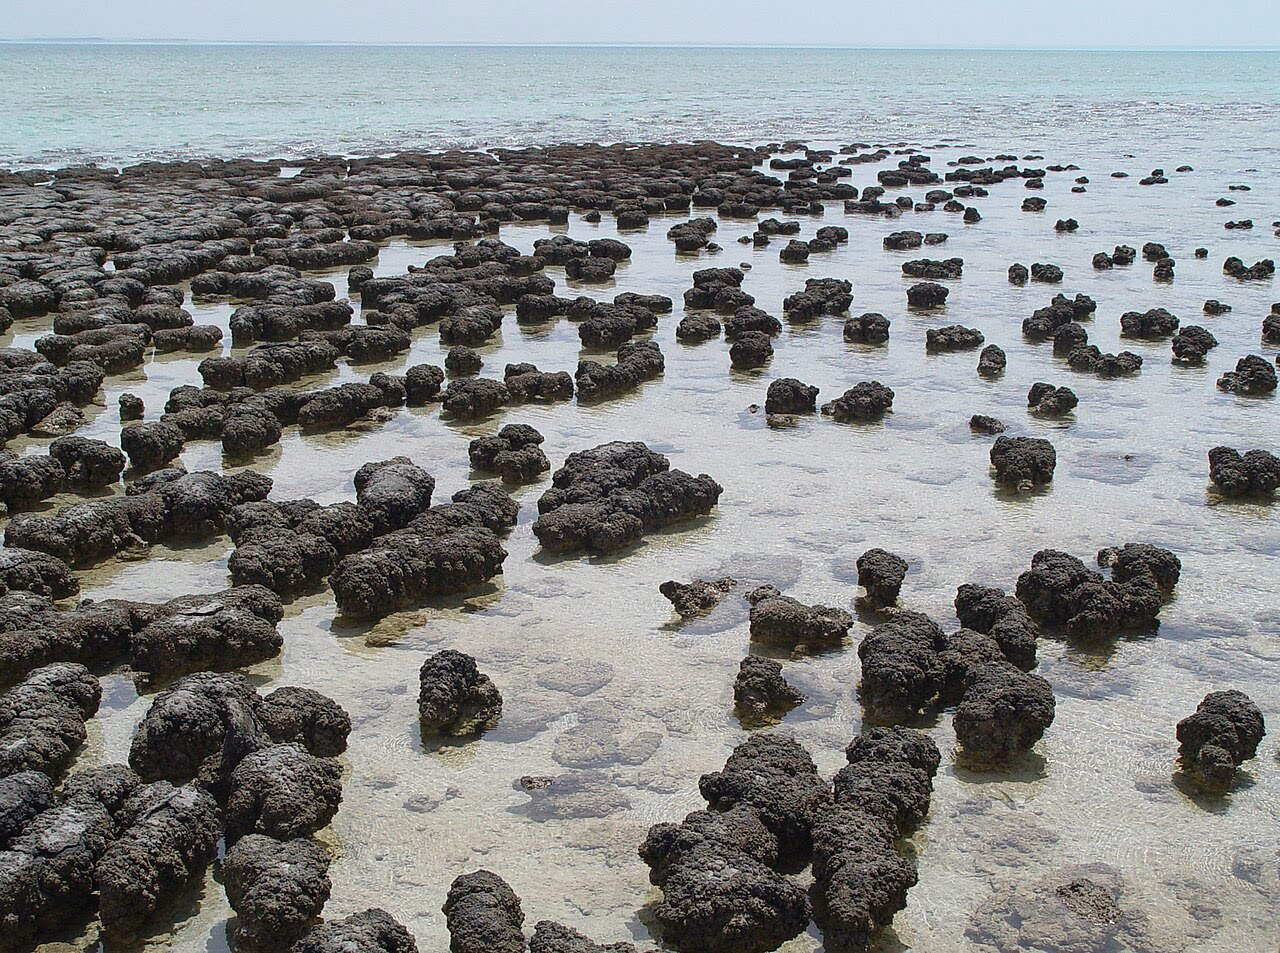
\includegraphics[width=0.6\linewidth]{images/book2/g12-shark-bay-stromatolites.jpg}

{\small \omterm{def:g12:early-earth:stromatolite}{Estromatólitos} vivos em Hamelin Pool, Shark Bay, Austrália
Ocidental. Fotografia Paul Harrison, CC~BY-SA~3.0 (Wikimedia Commons).}
\end{omfigure}
% ledger: photo:g12-shark-bay

As cianobactérias trouxeram uma novidade: uma fotossíntese que libera
oxigênio. Mas, por muito tempo, o oxigênio que elas produziam não ficou no
ar. Ele era consumido tão depressa quanto era produzido: pelo ferro
dissolvido no mar, pelo enxofre e pelo metano.

\section{A subida do oxigênio}

Antes do oxigênio, o ferro podia viajar dissolvido na água do mar como o
íon \ce{Fe^2+}. O oxigênio o transforma em ferro(III), que não se dissolve:
ele cai no fundo como um sedimento cor de ferrugem.

\begin{proposition}[O ferro capta oxigênio]\label{prop:g12:early-earth:iron}
O ferro(II) dissolvido é oxidado pelo oxigênio na água em hidróxido de
ferro(III), que precipita:
\[
  \ce{4Fe^2+ + O2 + 10H2O -> 4Fe(OH)3 + 8H+} .
\]
Cada molécula de oxigênio remove quatro íons de ferro dissolvido; enquanto
resta ferro dissolvido, o oxigênio produzido é consumido.
\end{proposition}
% ledger: earle:bif (ferrous iron oxidised to insoluble ferric iron)

\begin{proof}
Verifique o balanço. Ferro: 4 de cada lado. Oxigênio: $2 + 10 = 12$ à
esquerda, $4 \times 3 = 12$ à direita. Hidrogênio: $20$ à esquerda, $4 \times 3 + 8 =
20$ à direita. Carga: $4 \times (+2) = +8$ à esquerda, $8 \times (+1) =
+8$ à direita.
\end{proof}

\begin{definition}[Formação ferrífera bandada]\label{def:g12:early-earth:bif}
Uma \emph{formação ferrífera bandada}\index{formacao ferrifera bandada@formação ferrífera bandada}
é uma rocha sedimentar de camadas finas alternadas de óxidos de ferro, como a
hematita, e de chert, uma sílica de grão fino pobre em ferro. Quase todas
têm mais de 1.8 bilhão de anos.
\end{definition}
% ledger: earle:bif, holland06:stages

As \omterm{def:g12:early-earth:bif}{formações ferríferas bandadas} precisam de duas águas ao mesmo tempo: um
\omterm{def:g10:layered-ocean:thermocline}{oceano profundo} sem oxigênio, que transporta ferro dissolvido, e um mar
raso e ensolarado, onde as cianobactérias produzem oxigênio e o ferro
precipita. Elas são comuns em rochas de 2.4 a 1.8 bilhões de anos, e as das
Hamersley Ranges são ainda mais antigas. As \omterm{def:g12:early-earth:bif}{formações ferríferas bandadas}
são um minério de ferro comum.
% ledger: earle:bif, holland06:stages (Archean BIF, Hamersley), dbca:karijini

\begin{omfigure}
\begin{tikzpicture}[x=1cm, y=1cm, font=\scriptsize]
  % sea and floor
  \fill[omSea] (0,0) rectangle (11,4);
  \fill[omSea!45!white] (0,2.9) rectangle (11,4);
  \draw[omDef!60, line width=0.4pt, densely dashed] (0,2.9) -- (11,2.9);
  \node[anchor=north east, text=omDef] at (10.9,3.95) {água iluminada};
  \node[anchor=south east, text=omDef, align=right] at (10.9,0.12) {água profunda\\sem oxigênio,\\rica em \ce{Fe^2+}};
  % floor with layers
  \foreach \i/\c in {0/red!55!black, 1/black!20, 2/red!55!black, 3/black!20, 4/red!55!black, 5/black!20} {
    \fill[\c] (0,-0.12*\i) rectangle (11,-0.12*\i-0.12);
  }
  \draw[black!60] (0,0) -- (11,0);
  \node[anchor=west] at (11.1,-0.12) {óxido de ferro};
  \node[anchor=west] at (11.1,-0.36) {chert};
  \draw[black!50, line width=0.3pt] (11.05,-0.06) -- (10.6,-0.06);
  \draw[black!50, line width=0.3pt] (11.05,-0.30) -- (10.6,-0.30);
  % upwelling iron
  \foreach \x in {0.5,1.0,1.5} {
    \draw[-{Stealth}, omDef, line width=0.8pt] (\x,0.4) .. controls (\x+0.4,1.5) and (\x+0.6,2.2) .. (\x+0.9,2.85);
  }
  \node[text=omDef, anchor=west] at (2.3,1.3) {o \ce{Fe^2+} sobe};
  % cyanobacteria and oxygen
  \foreach \x in {3.8,4.4,5.0,5.6,6.2} {\fill[green!45!black] (\x,3.35) circle (0.07);}
  \node[anchor=south, text=green!35!black] at (5.0,3.47) {cianobactérias produzem \ce{O2}};
  % reaction
  \node[draw=black!40, fill=white, rounded corners=2pt, inner sep=2pt] at (5.4,2.45) {\ce{4Fe^2+ + O2 + 10H2O -> 4Fe(OH)3 + 8H+}};
  % falling rust
  \foreach \x/\y in {4.6/1.9, 5.0/1.5, 5.5/1.8, 5.9/1.2, 4.3/1.1, 5.2/0.7, 6.1/0.6} {\fill[red!60!black] (\x,\y) circle (0.06);}
  \draw[-{Stealth}, red!60!black, line width=0.6pt] (6.6,2.1) -- (6.6,0.25);
  \node[anchor=west, text=red!60!black, align=left] at (6.7,1.75) {o ferro(III) se deposita\\numa camada de ferrugem};
\end{tikzpicture}

{\small Como se forma uma \omterm{def:g12:early-earth:bif}{formação ferrífera bandada} (esquema, fora de
escala): o ferro dissolvido na água profunda, que não contém oxigênio, sobe
para o mar iluminado, onde o oxigênio produzido pelas cianobactérias o
transforma em ferro(III), que se deposita. Camadas ricas em ferro alternam
com camadas de chert.}
\end{omfigure}

Depois, o oxigênio começou a ficar no ar.

\begin{definition}[Grande Evento de Oxidação]\label{def:g12:early-earth:goe}
O \emph{Grande Evento de Oxidação}\index{Grande Evento de Oxidacao@Grande Evento de Oxidação} é o
intervalo, de cerca de \num{2.46} a cerca de \num{2.06} bilhões de anos
atrás, durante o qual o oxigênio livre se acumulou pela primeira vez na
atmosfera da Terra e nos mares rasos, chegando talvez a um décimo do seu
nível atual.
\end{definition}
% ledger: gumsley17:goe, holland06:stages (0.02-0.04 atm, about a tenth of 0.21)

As provas estão nas rochas. Alguns minerais, entre eles a pirita e a
uraninita, são destruídos pelo oxigênio; no entanto, grãos deles, rolados
pelos rios, são encontrados em sedimentos antigos, e os grãos de pirita
faltam nos que foram depositados depois da subida do oxigênio. Os isótopos do enxofre em rochas de mais de cerca de 2.45 bilhões de anos trazem uma
assinatura que só um ar com menos de um cem milésimo do oxigênio de hoje
pode deixar; há 2.09 bilhões de anos, ela desapareceu. E, nos continentes,
apareceram as \omterm{def:g12:early-earth:red-beds}{camadas vermelhas}.
% ledger: kasting25:indicators, pk02:anoxic, farquhar00:sulfur

\begin{definition}[Camadas vermelhas]\label{def:g12:early-earth:red-beds}
As \emph{camadas vermelhas}\index{camadas vermelhas} são rochas sedimentares
--- arenitos, siltitos, folhelhos --- coloridas de vermelho por uma película
de óxido de ferro(III), a hematita, sobre os seus grãos. Elas só se formam
onde há oxigênio bastante para oxidar o ferro.
\end{definition}
% ledger: kasting25:indicators (redbeds an oxygen indicator)

\begin{omfigure}
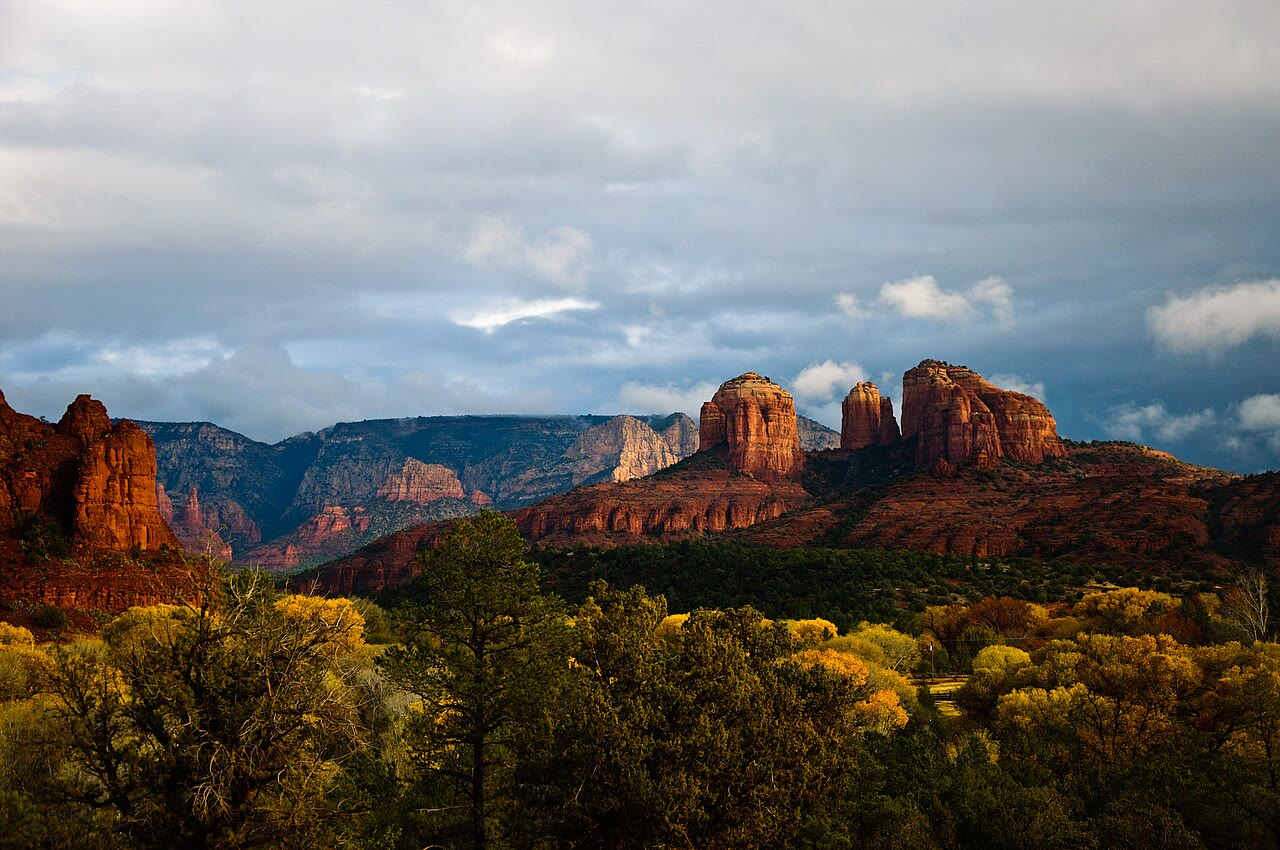
\includegraphics[width=0.66\linewidth]{images/book2/g12-sedona-red-beds.jpg}

{\small \omterm{def:g12:early-earth:red-beds}{Camadas vermelhas}: a Cathedral Rock perto de Sedona, no Arizona,
formada de arenitos vermelhos do Permiano. Fotografia Wendy from
Pennsylvania, CC~BY-SA~2.0 (Wikimedia Commons).}
\end{omfigure}
% ledger: photo:g12-sedona, azgs:cathedral (Permian Schnebly Hill Sandstone)

A formação das \omterm{def:g12:early-earth:bif}{formações ferríferas bandadas} praticamente cessou depois de
1.8 bilhão de anos atrás: nessa época, o \omterm{def:g10:layered-ocean:thermocline}{oceano profundo} também tinha
oxigênio bastante para deixar de transportar ferro. Durante o bilhão de anos
seguinte, o oxigênio mudou pouco; depois de 0.85 bilhão de anos atrás, ele
voltou a se acumular, em direção aos \qty{21}{\percent} de hoje.
% ledger: earle:bif, holland06:stages

\begin{method}[Ler uma linha do tempo geológica]\label{met:g12:early-earth:timeline}
\begin{enumerate}
  \item Descubra em que sentido o tempo corre no eixo, e a sua unidade
        (milhões ou bilhões de anos antes do presente).
  \item Localize os éons na faixa colorida, e leia os seus limites.
  \item Para cada evento, leia a sua data, ou o intervalo em que ele
        aconteceu, e diga que registro o data (um mineral, um fóssil, uma rocha).
  \item Calcule as durações por subtração, e compare-as com a \omterm{def:g12:age-of-the-earth:age}{idade da
        Terra}.
  \item Verifique a ordem: um efeito não deve vir antes da sua causa.
\end{enumerate}
\end{method}

\begin{omfigure}
\begin{tikzpicture}
\begin{axis}[omrecord, width=0.82\linewidth, height=6.2cm, ymode=log, xmin=0, xmax=4.6, ymin=1e-7, ymax=5,
  x dir=reverse, xlabel={tempo antes do presente (bilhões de anos)}, ylabel={oxigênio no ar (hoje $=1$)},
  xtick={0,0.5,...,4.5}, x tick label style={/pgf/number format/.cd, fixed, precision=1},
  ytick={1e-6,1e-4,1e-2,1}, ymajorgrids=true, xmajorgrids=false, clip=false]
% computed in figdata/grade-12/early_earth.py (schematic through the sourced bounds); ledger: holland06:stages, pk02:anoxic, gumsley17:goe, ics:base.Hadean, ics:base.Archean, ics:base.Proterozoic, ics:base.Paleozoic
\fill[omThm!12] (axis cs:2.46,1e-7) rectangle (axis cs:2.06,5);
\addplot[black, line width=1.2pt] table[x=t_Ga, y=pal] {figdata/out/grade-12-early_earth-oxygen.dat};
% eon band (ICS colours), below the axis
\fill[icsHadean] (axis cs:4.567,1.5e-7) rectangle (axis cs:4.031,4e-7);
\fill[icsArchean] (axis cs:4.031,1.5e-7) rectangle (axis cs:2.5,4e-7);
\fill[icsProterozoic] (axis cs:2.5,1.5e-7) rectangle (axis cs:0.5388,4e-7);
\fill[icsPhanerozoic] (axis cs:0.5388,1.5e-7) rectangle (axis cs:0,4e-7);
\node[font=\tiny, text=white] at (axis cs:4.30,2.45e-7) {Hadeano};
\node[font=\tiny, text=white] at (axis cs:3.27,2.45e-7) {Arqueano};
\node[font=\tiny, text=white] at (axis cs:1.52,2.45e-7) {Proterozoico};
% events
\draw[omDef, line width=0.6pt] (axis cs:4.4,4e-7) -- (axis cs:4.4,3e-3);
\node[font=\scriptsize, text=omDef, anchor=south west] at (axis cs:4.4,3e-3) {zircões, água};
\draw[omMeth, line width=0.6pt] (axis cs:3.43,4e-7) -- (axis cs:3.43,1.2e-6);
\node[font=\scriptsize, text=omMeth, anchor=south] at (axis cs:3.43,1.2e-6) {primeiros estromatólitos};
\draw[red!60!black, line width=3pt] (axis cs:2.4,3e-6) -- (axis cs:1.8,3e-6);
\node[font=\scriptsize, text=red!60!black, anchor=north] at (axis cs:2.16,2.4e-6) {formações ferríferas bandadas};
\node[font=\scriptsize, text=omThm, anchor=south, align=center] at (axis cs:2.26,1.2) {Grande Evento\\de Oxidação};
\node[font=\scriptsize, anchor=south] at (axis cs:3.2,1.3e-5) {menos de $10^{-5}$ do atual};
\node[font=\scriptsize, anchor=south] at (axis cs:1.4,0.12) {cerca de um décimo};
\end{axis}
\end{tikzpicture}

{\small O oxigênio no ar ao longo do tempo (esquema, escala logarítmica): a
curva liga os limites medidos e esconde os altos e baixos do registro real.
O intervalo sombreado é o \omterm{def:g12:early-earth:goe}{Grande Evento de Oxidação}; a barra vermelha marca
a época em que as \omterm{def:g12:early-earth:bif}{formações ferríferas bandadas} eram comuns, de 2.4 a 1.8
bilhões de anos atrás. Éons segundo a Tabela Cronoestratigráfica
Internacional.}
\end{omfigure}

\section{Exercícios}

\begin{exercise}[$\star$]\label{exo:g12:early-earth:1}
Dê a palavra: (a) a liberação dos gases dissolvidos no magma; (b) um
montículo em camadas construído por um tapete microbiano; (c) uma rocha de
camadas alternadas de óxido de ferro e de chert; (d) rochas sedimentares
coloridas pela hematita; (e) o intervalo em que o oxigênio se acumulou pela
primeira vez no ar.
\end{exercise}

\begin{exercise}[$\star$]\label{exo:g12:early-earth:2}
Ponha em ordem, da mais antiga: o fim da maioria das \omterm{def:g12:early-earth:bif}{formações ferríferas
bandadas}; os primeiros \omterm{def:g12:early-earth:stromatolite}{estromatólitos} da Pilbara; os zircões que mostram água
líquida; as \omterm{def:g12:early-earth:bif}{formações ferríferas bandadas} das Hamersley Ranges; o fim do
\omterm{def:g12:early-earth:goe}{Grande Evento de Oxidação}.
\end{exercise}

\begin{exercise}[$\star$]\label{exo:g12:early-earth:3}
Usando a lei da luminosidade, calcule a luminosidade do Sol no seu
nascimento, como fração da de hoje. Em que porcentagem ele era menos
brilhante?
\end{exercise}

\begin{exercise}[$\star$]\label{exo:g12:early-earth:4}
Grãos de pirita rolados pelos rios são encontrados em sedimentos antigos, mas
não nos que foram depositados depois da subida do oxigênio. O que isso lhe
diz sobre o ar na época dos sedimentos antigos? Por quê?
\end{exercise}

\begin{exercise}[$\star$]\label{exo:g12:early-earth:5}
Dê os nomes dos dois gases mais abundantes liberados pelos vulcões, e diga o
que aconteceu com cada um na Terra jovem.
\end{exercise}

\begin{exercise}[$\star\star$]\label{exo:g12:early-earth:6}
Calcule a luminosidade do Sol e a \omterm{def:g10:habitable-planet:equilibrium-temperature}{temperatura de equilíbrio} da Terra (hoje
\qty{255}{K}, \omterm{def:g10:earth-energy-budget:albedo}{albedo} inalterado) há 3 bilhões de anos e há 2.45 bilhões de
anos, tomando $t_\odot = 4.567$ bilhões de anos.
\end{exercise}

\begin{exercise}[$\star\star$]\label{exo:g12:early-earth:7}
Quanto oxigênio é necessário para precipitar \qty{1}{kg} de ferro dissolvido
como hidróxido de ferro(III)? (Massas molares: ferro \qty{55.85}{g/mol},
oxigênio \qty{16.00}{g/mol}.)
\end{exercise}

\begin{exercise}[$\star\star$]\label{exo:g12:early-earth:8}
Usando a linha do tempo, (1) quanto tempo durou o \omterm{def:g12:early-earth:goe}{Grande Evento de Oxidação}?
(2) Durante que fração da história da Terra quase não houve oxigênio no ar?
(3) Quanto tempo depois dos primeiros \omterm{def:g12:early-earth:stromatolite}{estromatólitos} o oxigênio começou a se
acumular?
\end{exercise}

\begin{exercise}[$\star\star$]\label{exo:g12:early-earth:9}
Uma \omterm{def:g12:early-earth:bif}{formação ferrífera bandada} e uma camada vermelha contêm, as duas, óxido
de ferro(III). O que cada uma lhe diz sobre o oxigênio, e onde: no mar
profundo, no mar raso, no ar?
\end{exercise}

\begin{exercise}[$\star\star$]\label{exo:g12:early-earth:10}
Onde se podem ver \omterm{def:g12:early-earth:stromatolite}{estromatólitos} vivos hoje? O que a água tem de especial
ali, e como um \omterm{def:g12:early-earth:stromatolite}{estromatólito} cresce camada após camada?
\end{exercise}

\begin{exercise}[$\star\star$]\label{exo:g12:early-earth:11}
O oxigênio representa \qty{21}{\percent} do ar de hoje. Que porcentagem ele
representava quando estava (1) a um cem milésimo do nível de hoje; (2) a um
décimo do nível de hoje?
\end{exercise}

\begin{exercise}[$\star\star\star$]\label{exo:g12:early-earth:12}
Há quatro bilhões de anos, que \omterm{def:g10:earth-energy-budget:albedo}{albedo} teria dado à Terra a \omterm{def:g10:habitable-planet:equilibrium-temperature}{temperatura de
equilíbrio} de hoje, \qty{255}{K}, sob o Sol jovem ($L = 0.741\,L_\odot$,
\omterm{def:g10:earth-energy-budget:albedo}{albedo} de hoje 0.294)? É provável que um planeta com um oceano, nuvens e um
pouco de gelo tenha sido tão escuro? Qual é a outra saída?
\end{exercise}

\begin{exercise}[$\star\star\star$]\label{exo:g12:early-earth:13}
Hoje o efeito estufa aquece a superfície da Terra de 255 para
\qty{288}{K}. Há quatro bilhões de anos, a \omterm{def:g10:habitable-planet:equilibrium-temperature}{temperatura de equilíbrio} era de
cerca de \qty{237}{K}. (1) Quantos kelvins de aquecimento por efeito estufa
eram então necessários para chegar a \qty{273}{K}? E a \qty{288}{K}?
(2) Compare com o de hoje. (3) Um cálculo clássico precisa de cerca de
\qty{0.1}{bar} de gás carbônico, com um pouco de metano; compare com a
pressão da atmosfera inteira de hoje, cerca de \qty{1}{bar}.
\end{exercise}

\begin{exercise}[$\star\star\star$]\label{exo:g12:early-earth:14}
Uma assinatura especial dos isótopos do enxofre só pode ser produzida, e
conservada nos sedimentos, quando o ar contém menos de $10^{-5}$ do oxigênio
de hoje. Ela é encontrada em rochas de mais de 2450 milhões de anos, e não em
rochas de menos de 2090 milhões de anos. (1) O que você conclui sobre o
oxigênio antes de 2450 milhões de anos atrás? E depois de 2090 milhões de
anos? (2) Isso é coerente com as datas do \omterm{def:g12:early-earth:goe}{Grande Evento de Oxidação}?
\end{exercise}

\begin{exercise}[$\star\star\star$]\label{exo:g12:early-earth:15}
O impacto que formou a Lua aconteceu cerca de 60 milhões de anos depois que
o Sistema Solar começou a se formar, início que a datação dos primeiros
sólidos situa há 4567 milhões de anos. (1) Por volta de quando aconteceu o impacto?
(2) Os zircões mais antigos têm \num{4404} milhões de anos. No máximo quanto
tempo depois do impacto a Terra já tinha uma crosta sólida e água líquida?
\end{exercise}
% ledger: nasa:moon-formation, connelly12:cai, wilde01:4404

\begin{problem}[{Problema de fim de semana --- o Sol jovem e fraco}]
\label{pb:g12:early-earth:1}
% ledger: gough81:luminosity, connelly12:cai, earth:TSI, earth:albedo, earth:Tsurf, feulner12:fys, allwood06:spc, dbca:karijini, wilde01:zircon
% values (early_earth.py): L_4Ga 0.7406, S_4Ga 1007.9, Teq_today 255.1, Teq_4Ga 236.7, albedo_needed 0.047
O Sol tem \num{4.567} bilhões de anos. A sua luminosidade quando ele tinha $t$
anos era $L(t) = L_\odot/\bigl(1 + \tfrac25 (1 - t/t_\odot)\bigr)$. Hoje,
a Terra recebe \qty{1361}{W/m^2} de luz do Sol, reflete uma fração 0.294
dela, e tem uma \omterm{def:g10:habitable-planet:equilibrium-temperature}{temperatura de equilíbrio} de \qty{255}{K}; a sua temperatura
média de superfície é de \qty{288}{K}.

\medskip
\noindent\textbf{Parte I --- O Sol há quatro bilhões de anos.}
\begin{enumerate}
  \item Que idade tinha o Sol há quatro bilhões de anos?
  \item Calcule $1 - t/t_\odot$ nessa época.
  \item Calcule a sua luminosidade como fração da de hoje.
  \item Que luz do Sol a Terra recebia, em \unit{W/m^2}?
  \item Em que porcentagem o Sol era menos brilhante que hoje?
\end{enumerate}

\medskip
\noindent\textbf{Parte II --- A temperatura de equilíbrio.}
\begin{enumerate}[resume]
  \item Escreva a \omterm{def:g10:habitable-planet:equilibrium-temperature}{temperatura de equilíbrio} em função da luz do Sol $S$.
  \item Mostre que, com o \omterm{def:g10:earth-energy-budget:albedo}{albedo} inalterado, a temperatura varia como
        $S^{1/4}$.
  \item Calcule $0.741^{1/4}$.
  \item Calcule a \omterm{def:g10:habitable-planet:equilibrium-temperature}{temperatura de equilíbrio} há quatro bilhões de anos.
  \item Converta-a em graus Celsius.
\end{enumerate}

\medskip
\noindent\textbf{Parte III --- Indícios de água líquida.}
\begin{enumerate}[resume]
  \item O que mostram os zircões de 4.4 bilhões de anos?
  \item Em que tipo de água cresceram os \omterm{def:g12:early-earth:stromatolite}{estromatólitos} da Pilbara, de
        \num{3430} milhões de anos?
  \item Que rochas das Hamersley Ranges, depositadas no mar há mais de
        2.5 bilhões de anos, precisam de água líquida?
  \item Sem efeito estufa, o oceano teria congelado há quatro bilhões de
        anos? Por quê?
  \item Enuncie a contradição que isso revela, e dê o seu nome.
\end{enumerate}

\medskip
\noindent\textbf{Parte IV --- O aquecimento por efeito estufa necessário.}
\begin{enumerate}[resume]
  \item Quantos kelvins o efeito estufa de hoje acrescenta?
  \item Quantos eram necessários há quatro bilhões de anos para manter a
        superfície média acima de \qty{273}{K}?
  \item Que \omterm{def:g10:earth-energy-budget:albedo}{albedo} teria dado \qty{255}{K} sem nenhum efeito estufa
        adicional? Isso é plausível?
  \item Que gás teria fornecido a maior parte do aquecimento adicional, e
        que outro gás pode ter ajudado?
  \item Resuma: qual era a \omterm{def:g10:habitable-planet:equilibrium-temperature}{temperatura de equilíbrio} da Terra há quatro
        bilhões de anos?
\end{enumerate}
\end{problem}
